\documentclass{article}
\usepackage[utf8]{inputenc}
\usepackage{fancyhdr}
\usepackage[top=1.25in, bottom=1.25in, right=1in, left=1in]{geometry}
\usepackage{graphicx}
\usepackage{amsmath,amsfonts,amssymb,amsthm}
\PassOptionsToPackage{hyphens}{url}
\usepackage{hyperref}

\hypersetup{colorlinks=true, linkcolor=blue, urlcolor=blue}

\usepackage{etoolbox}
\makeatletter
\patchcmd\g@matrix
 {\vbox\bgroup}
 {\vbox\bgroup\normalbaselines}% restore the standard baselineskip
 {}{}
\makeatother

\pagestyle{fancy}
\fancyhf{}
\rhead{Introduction to Data Science}
\lhead{Predicting Electricity Spot Price}
\rfoot{Page \thepage}
\makeatletter
\renewcommand{\@seccntformat}[1]{}
\makeatother 

%% Theorems etc. %%%%%%%%%%%%%%
%\swapnumbers
\numberwithin{equation}{section}

\makeatletter
\let\c@equation\c@subsection
\makeatother

\title{%
	Predicting Electricity Spot Price\\
	\large Introduction to Data Science Course Project}
\author{Ville Pirsto, Emil Tigerstedt, Ahsan Abbas}

\begin{document}

% Titlepage separately
\begin{titlepage}
	\maketitle
	\thispagestyle{empty}
\end{titlepage}

\tableofcontents
\clearpage

% ---- Introduction ----
\section{Introduction}
This project was done as a part of "Introduction to data science" course in Helsinki University. The focus of this project was to predict the electricity spot prices in Finland, idelly for a longer time horizon that is typically available to the consumer. In Finland, the spot electricity prices for the next day are published typically on the previous day after noon, so the spot price horizon is always less than 36 hours. 

Such a short price horizon does not allow very long-term planning of electricity consumption. Moreover, there is a psychological effect in play due to uncertainty about the upcoming prices; will I minimize my electricity bill if I do the chores that consume a lot of energy during the price minimum of the current horizon, or will there be even cheaper electricity before I really need to do these chores? One concrete example is charging of ones electric vehicle. Let's say you are planning to drive and see your friends and/or family in the upcoming weekend and it is now monday. You know that you would like to have the battery charged to near-full before your departure on friday afternoon. Should you top up your car battery during the minimum price of the current price horizon, or wait and see if you can save money by postponing until later in the week?

We attempted to address this problem by developing a prediction model for the spot electricity price with longer time horizon. In the spirit of experimentation, we did not got for the most obvious predictor variable there are, such as electricity production from the most dominant sources of energy in Finland (for example, wind and nuclear), or energy exported/imported from other countries. Instead, we attempted to tackle this prediction problem by utilizing more "indirect" predictors.

This report will walk through our project by utilizing the project work canvas. First, the filled canvas is presented, followed by brief discussion on each of the tiles in the canvas.

\clearpage
% ---- Canvas ----
\section{Project Work Canvas and Practicalities}
Figure \ref{fig1} showcases the canvas filled in the beginning of the course. While brief in its contents and merely reflecting the initial ideas we had for the project at the beginning of the course, it provides the structure of this report as well. In the following sections, the parts of the canvas are addressed in retrospective.

Regarding the practicalities of the project, we used Telegram app as our main communication platform. Moreover, we had weekly face-to-face meetings on the campus where we discussed the progress last week and planned for the upcoming week. The "minutes of meeting" for each week containing the plans for next week in a condensed format were saved into the project repository in Github. Right at the beginning of the project, we decided to do the implementation with Python and using Jupyter notebook as the platform that enables quick testing of different approaches and ease of sharing results between team members.

The repository of the project can be found from \href{https://github.com/pirstov/Intro_to_DS_project}{\textbf{here}}.



\begin{figure}[htb]
	\centering
	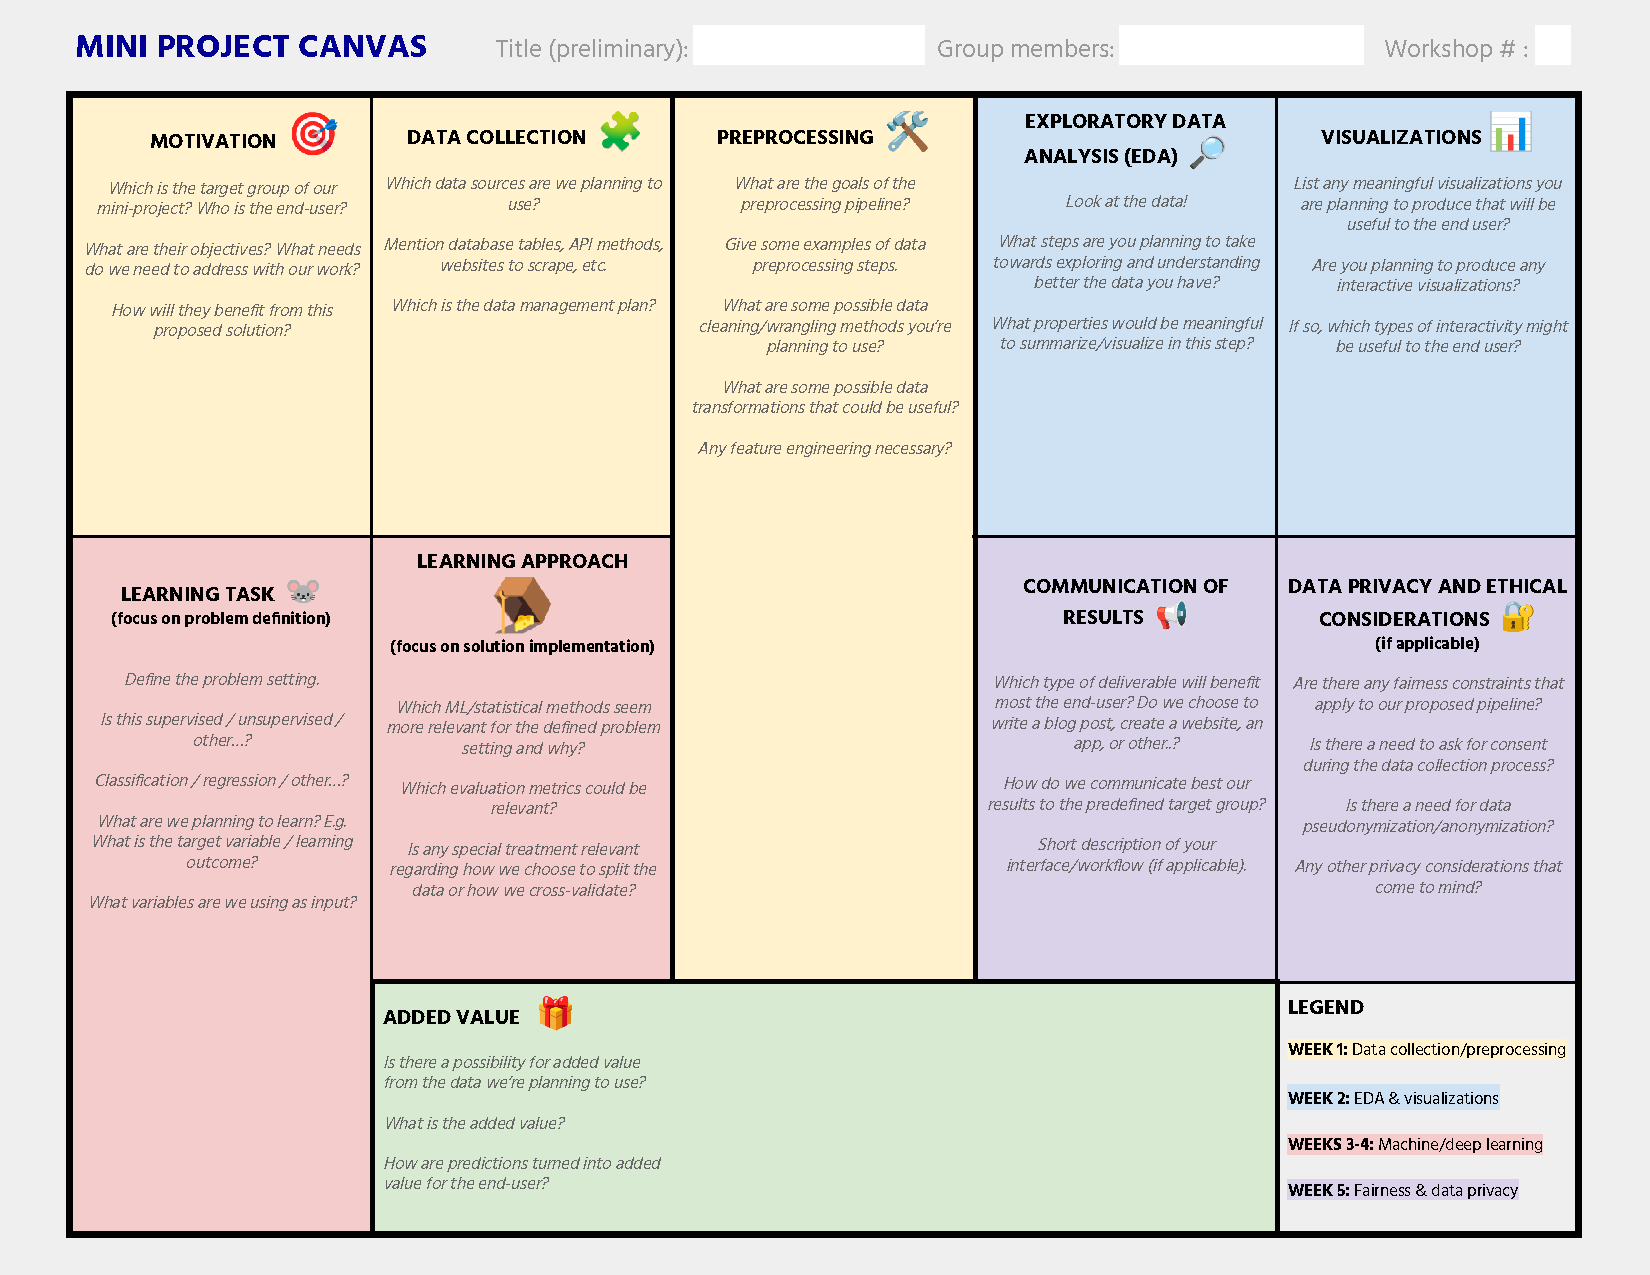
\includegraphics[width=1\textwidth]{./mini_project_canvas.pdf}
	\caption{Canvas used for project planning.}
	\label{fig1}
\end{figure}

\clearpage
% ---- Data Collection and Preprocessing ----
\section{Data Collection and Preprocessing}
Firstly, we gathered historical spot price data for Finland from \href{https://porssisahko.net/tilastot}{this website}. Additionally, we collected weather data from the \href{https://www.ilmatieteenlaitos.fi/avoin-data/}{Finnish Meteorological Institute} and electricity consumption and production data from Fingrid's open data platform (\href{https://data.fingrid.fi/en/datasets/124}{here} and \href{https://data.fingrid.fi/en/datasets/192}{here}, respectively). All datasets were in Excel format and were downloaded using specific start and end dates as parameters. The data was then imported into a Jupyter notebook using Python, where we created a Pandas DataFrame for each dataset. We then proceeded to preprocess the data to ensure a consistent structure across all datasets.

Preprocessing began with the spot price data, which consisted of two columns: '\verb|Aika|' (time) and '\verb|Hinta (snt/kWh)|' (price). We adjusted the time column so that prices were aligned with every even hour, and applied this format to the other datasets as well. 

The weather data was acquired from Kalajoki weather station, as multiple wind farms neighbour it. In the weather data, the year, month, day, and hour were originally in separate columns, so we combined them into a single datetime object. Since the observations were already recorded hourly, no further significant modifications were needed. Different elements of the weather data, such as mean temperature, were stored in separate columns, similar to the structure of the electricity price data.

The electricity consumption and production data, retrieved from the same open data platform, had similar structures. Both datasets included two time-related columns—'\verb|startTime|' and '\verb|endTime|'—along with a column for production or consumption values. We consolidated the two time columns into one, following the same approach used for the weather data. Additionally, the time column still contained extraneous characters, which were cleaned up, and the values were converted into datetime objects.

The main difference between the production and consumption datasets was the frequency of observations: production data was recorded every three minutes, while consumption data was recorded hourly. To standardize the data, we calculated the hourly average for the production data to match the required format.

Once all the datasets were in the correct format, we merged them into a comprehensive dataframe. We then performed imputation, replacing any missing values with the column medians. Finally, we added one more input variable: a boolean variable indicating whether the date of an observation fell on a public holiday. The public holiday dates were sourced from \href{https://www.officeholidays.com/countries/finland/2021}{this website}.

All the data collection and preprocessing described above was carried out in a single Jupyter notebook. In addition, we created three separate Jupyter notebooks, each dedicated to handling one API. These APIs were used to fetch weather, electricity consumption, and electricity production forecasts for the upcoming days. The API used for the weather forecast is available in \href{https://api.open-meteo.com/v1/forecast}{here}, and the data retrieved required no significant preprocessing. Electricity consumption and production predictions were collected via APIs available on the same Fingrid open data platform as the historical data. Since the prediction data had a structure very similar to the historical data, we were able to reuse the preprocessing methods to bring the predictions into the desired format.

% ---- EDA and Visualizations ----
\section{Exploratory Data Analysis and Visualizations}

We began the exploratory data analysis by creating pair plots using functions from the Seaborn library, which generated scatter plots and kernel density estimate plots for each variable pair. To make these plots more informative, we added a hue to categorize data points as either 'day' or 'night.' This was achieved by introducing a new column, time_of_day, with values assigned based on the hour of each observation: data points from 6:00 to 18:00 were labeled as day, while those from 18:00 to 6:00 were labeled as night. The pair plots revealed few notable patterns except for one clear trend: electricity consumption was consistently lower at night than during the day.

In addition to pair plots, we visualized each variable with line plots, where the y-axis represented observed values and the x-axis represented time. These line plots highlighted clear seasonal patterns, with temperatures naturally peaking in the summer months, while electricity production and consumption were significantly higher in the winter.

We then used box plots and the Pandas describe function to identify outliers. Outliers were detected in the average temperature and electricity price columns, so we removed the observations containing these outliers to ensure they would not skew the analysis.

Additional EDA techniques included autocorrelation plots, the corr function from Pandas to examine variable correlations, and further line plots to visualize trends across different time intervals - daily, weekly, and monthly - to support our assessment of seasonal patterns. Correlation analysis revealed that electricity price was most influenced by wind speed and electricity consumption. Wind speed had a negative correlation with electricity prices, while consumption showed a positive correlation.

% ---- Learning ----
\section{Learning to Predict Electricity Spot prices}
During the project, we focused on three different approaches to predict the electricity spot price. Our initial plan was to apply time series modeling to fit a model that would capture both the seasonality of the prices both day- and year-wise, since seasonality was clearly visible in the input variables as well as the predicted varible during the data analysis stage. Seasonality was captured quite well by to model, but it was not able to capture the significant day-to-day variations that occur in the spot prices due to various reasons. One major contributing factor here was probably the choice of predictors, but we wanted to keep the number of inputs low. Nevertheless, after considerable effort in tuning and trying different time series models, we had to concede on this front.

Our second approach was to use \verb|XGBoost| machine learning algorithm to do the predictions. This selection was based on previous good experiences with this method. \verb|XGBoost| is based on gradient-boosted decision trees. However, we quickly found out that this approach yielded lower accuracy than a time series models, and decided to continue searching for another method.

Finally, motivated by the exercises in the course, we utilized the \verb|TPOT| library to suggest us a model. \verb|TPOT| proposed to apply random forest algorithm, and we tried it. As predicted by \verb|TPOT|, it turned out to yield the best prediction accuracy out of the models we had tried so far, and consequently, we decided to use it. This model was then saved to be used by the job application using Python library \verb|joblib| to avoid having to re-train every time someone accessess the website. In practice, this model should somehow be updated from time to time, but such implementation was outscoped from this project.

One hard constraint for prediction was arising from the availability of forecasts for input variables. All the methods required forecast information for the hours we wanted to predict for, but many of the input variables we considered throughout the project did not have forecasts available at all, or the forecast horizon was relatively short. In the case of the data we had selected, forecasts were available for the next 21 hours, creating a limit for the horizon of prediction. Input variable selection so that the goal of achieving good prediction accuracy while having access to long-term predictions is one of the possible future improvement topics.

% ---- Communciation of Results ----
\section{Communication of Results}
The results were communicated through a webpage found \href{https://connect.posit.cloud/AhsanAbbas101/content/0192c52c-7101-3655-bc34-0e4733cd46de}{here}. It contains an interactive graph for the user to examine the electricity spot price predictions for the upcoming 21 hours. The graph can present the data as either line or bar plot, selectable by the user in the settings column found on the left. Moreover, the graph can be zoomed, cursor for data point values is available, and the graph can even be saved. The user can also view the true spot prices to compare the accuracy of the method by checking a box on the left column of the webpage. This simple and clean implementation should enable the user to effortlessly see the spot price predictions for the future in a quick glance to make decisions regarding her/his electricity consumption.

The webpage implementation was based on the Python library \verb|shiny|. This allowed us to create the web user interface purely through Python. The historical data was stored to a cloud database using \verb|sqlite| in Python, and forecast data was accessed through the API methods mentioned in the data collection and preprocessing section. The prediction model was loaded from the stored joblib file.




% ---- Summary ----
\section{Summary}
As it turns out, predicting electricity spot prices is difficult. The machinery behind the price fluctuations is complex and can not be explained through weather and directly related predictors. Indeed, one needs to consider not only national, but international weather and electricity markets. Moreover, thorough coverage of the various significant electricity production forms in Finland should be included in the mix. Last, but not least, forecasts of the variables used in the prediction should be available, creating further limitations to the applicability of data. Considering the future continuation of this project, one might try to add more predictors that are directly tied to the electricity market and have long-term forecasts readily available. Other approach is to consider prediction methods relying on another type of input data so that such forecasts would not be required.

Nevertheless, the participants considered the project successful. Each one learned something new along the way. Some highlights of the themes we learned about include data preprocessing and formatting for learning, familiarizing ourselves with different artificial intelligence models, learning to use APIs for data collection, getting comfortable with version control, and planning short business pitches. Last, but not the least, we also improved our collaboration and communication skills.



% ----------------------------------------------------------------
\iffalse
\begin{figure}[htb]
\centering
\includegraphics[width=.5\textwidth]{./largestEigenvalue.eps}
\caption{Suurimman ominaisarvon approksimaatiovirheen itseisarvo $i$:n funktiona.}
\label{fig1}
\end{figure}
\fi

\end{document}
